\documentclass[pdftex,letterpaper,12pt]{report}
\usepackage{thesis}
\usepackage{amsmath}
\usepackage{amssymb}
\usepackage{amsthm}
\usepackage{mathtools}
\usepackage{bm}
\usepackage{gensymb}
\usepackage{wasysym}
\usepackage{mathtools}
\usepackage{physics}
\usepackage{empheq}
\usepackage{cases}
\usepackage{rotating}
\usepackage{subfig}
\usepackage{caption}
\captionsetup{labelfont=bf} 
\captionsetup[subfloat]{position=top,singlelinecheck=off,justification=raggedright,font=bf,labelfont=large,labelformat=simple,captionskip=-2mm}
\usepackage{float}
\usepackage{enumitem} 
\usepackage[toc,page]{appendix}






\begin{document}
	
\begin{subequations}
	\begin{gather}
	\frac{\partial M_{x}(t)}{\partial t}=\gamma\left(\boldsymbol{M(t)}\times \boldsymbol{B(t)}\right)_{x}-\frac{M_{x}(t)}{T_{2}^{*}}\\
	\frac{\partial M_{y}(t)}{\partial t}=\gamma\left(\boldsymbol{M(t)}\times \boldsymbol{B(t)}\right)_{y}-\frac{M_{y}(t)}{T_{2}^{*}}\\
	\frac{\partial M_{z}(t)}{\partial t}=\gamma\left(\boldsymbol{M(t)}\times \boldsymbol{B(t)}\right)_{z}-\frac{M_{z}(t)}{T_{1}}
	\end{gather}
\end{subequations}

\begin{equation}
S=A\omega \sin{\alpha(t)}=A\omega \frac{B_{1}}{\sqrt{B_{1}^{2}+(B(t)-\omega/\gamma)^{2}}}
\end{equation}

well under 100\%.
$k_{se}^{K}=(7.46\pm0.62)\times10^{-20}$ cm^{3}/s

\begin{equation}
\frac{1}{\gamma_{se}}\approx 15.9 hrs
\end{equation}

\begin{table}[t!]
	\begin{center}
		\caption{ Pressure broadening of Rb D$_{1}$ lines by $^{3}$He, $^{4}$He and N$_{2}$. The broadening and shifting density coefficients are listed. The 4th and 6th columns are the temperature dependence for He and N$_{2}$, respectively. All coefficients are given for 353 K, values for different temperatures can be calculated with the temperature dependence.}
		\label{PBCoef}
		\begin{tabular}{ c c c c c c}
			\hline \hline
			& $^{4}$He & $^{3}$He & Temp. depen. & N$_{2}$ & Temp. depen.\\ 
			D$_{1}$ full width & 18.0$\pm$0.2 & 18.7$\pm$0.3 & T$^{0.05\pm0.05}$ & 17.8$\pm$0.3 & T$^{0.3}$\\ 
			(GHz/amg) &&&&& \\
			D$_{1}$ line shift & 4.3$\pm$0.1 & 5.64$\pm$0.15 & T$^{1.1\pm0.1}$ &
			-8.25$\pm$0.15 & T$^{0.3}$ \\ 
			(GHz/amg) &&&&& \\ \hline \hline
		\end{tabular}
	\end{center}
\end{table}

The coefficients of pressure broadening for $^{3}$He, $^{4}$He and N$_{2}$ are listed in Table~\ref{PBCoef}.

\begin{figure}[t!]
	\centering
	\resizebox{0.91\textwidth}{!}{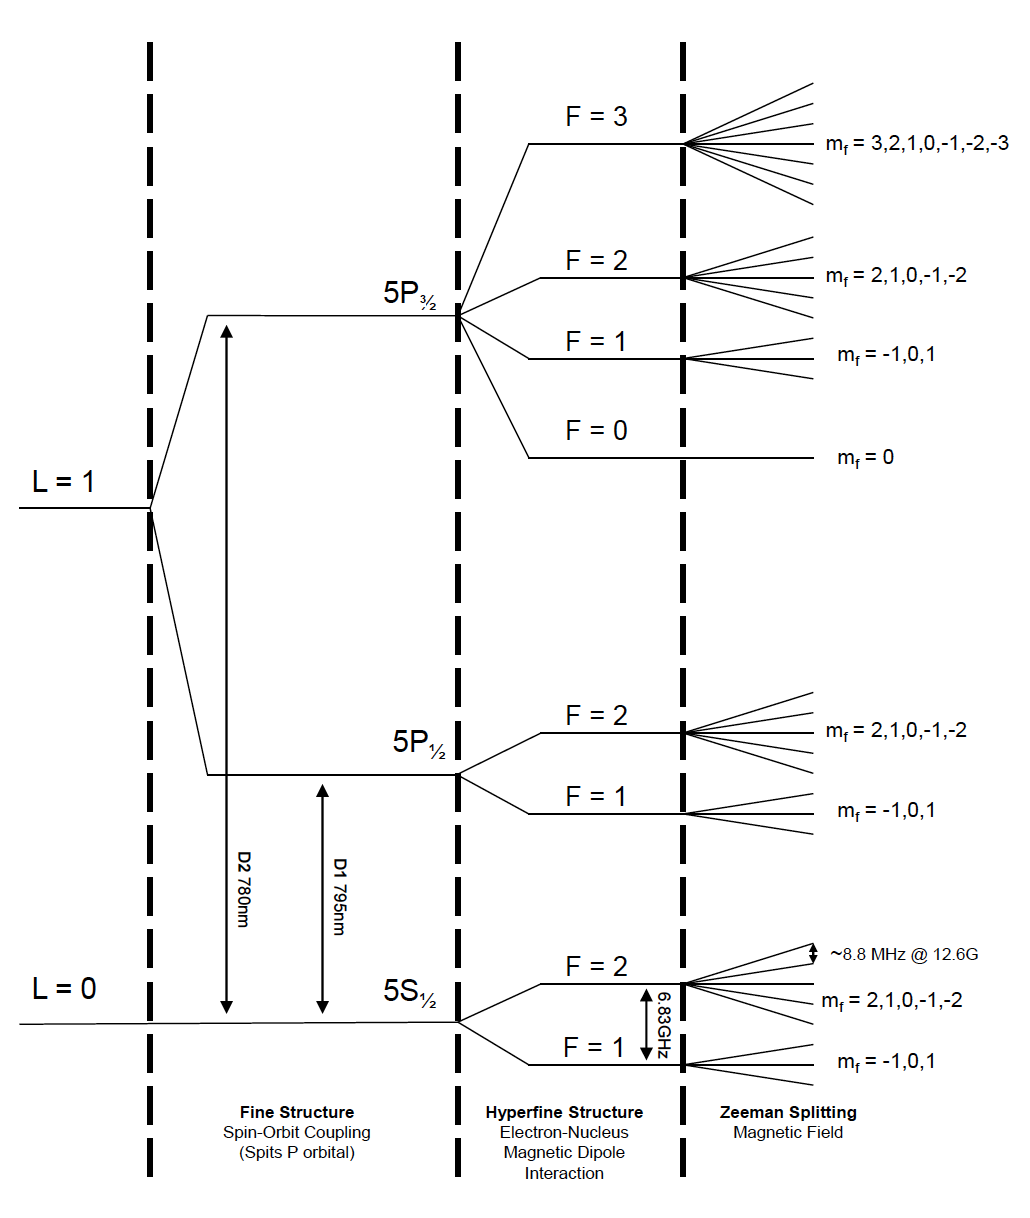
\includegraphics{RbEnergyLevels.png}}
	\caption{{\bf Level Diagram of $^{87}$Rb. The splittings are not to scale. Adapted from Dolph's PhD thesis.}}
	\label{RbEnergyLevels}
\end{figure}

The energy levels of $^{87}$Rb are shown in Fig.~\ref{RbEnergyLevels}.
where $\Gamma_{A}$ is the pressure dependent FWHM, $\Gamma_{A}\approx 0.04nm/amg \cdot [^{3}He]$.

\addcontentsline{toc}{chapter}{Bibliography}
\bibliography{ref}

\end{document}